The robot base comprises of four legs, with two on each side that are concentric. On either side, two of the legs are connected via a revolute joint and is concentric. The front wheels have a revolute joint connected to the wheels so that the robot can steer left or right. To have the robot at the same height, the rear wheels have the same joint however it is fixed. The robot arm that is attached has four degrees of freedom.\\

Modeling the robot is split into the vehicle and arm separately. With this method, both models can be configured and tested properly in Gazebo in order to use tele-op on individual joints. Figure~\ref{sample_return_rover:robot_design:srr_cad} shows the rover modeled in SolidWorks. Table~\ref{sample_return_rover:robot_design:srr_dimensions} lists the dimensions of the robot and links. Figure~\ref{sample_return_rover:robot_design:arm_model} and Figure~\ref{sample_return_rover:robot_design:arm_side} are images of the arm for reference.

\begin{table}[H]
	\centering
	\begin{tabular}{|c|c|} 
		\hline 
		\textit{Link} & \textit{Length} \\
		\hline
		Chassis Length & 18in \\
		Chassis Width & 12in \\
		Chassis Max Height & 7in \\
		Leg from Center Joint & 8.6in \\
		Length of Steering Link & 5.25in \\ 
		Wheel Diameter & 7.5in \\
		Wheel Track & 19.3in \\
		Wheelbase & 13.9in \\
		\hline
	\end{tabular}
	\caption{Table of Dimensions of the Rover}
	\label{sample_return_rover:robot_design:srr_dimensions}
\end{table}

\begin{figure}[H]
	\centering
	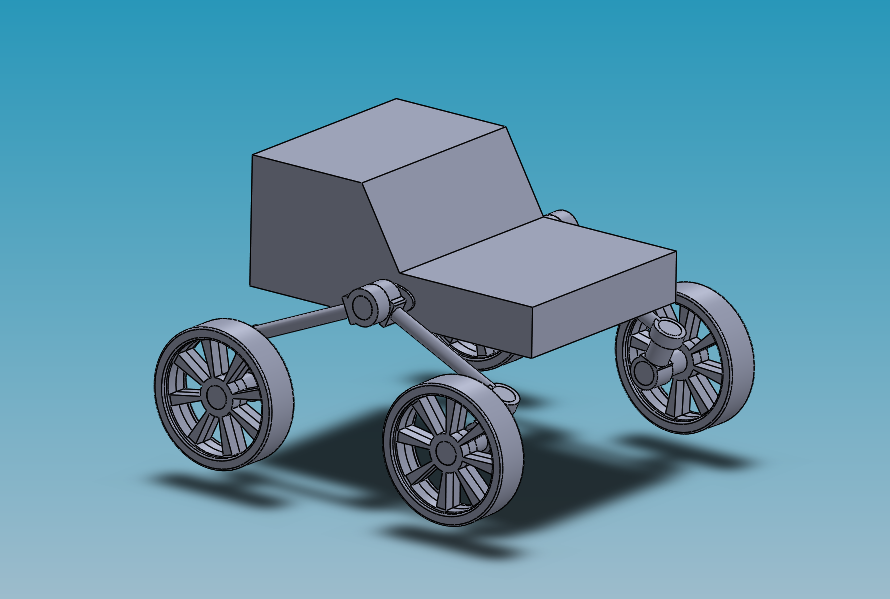
\includegraphics[scale=0.45]{sections/robot-design/images/SRR_model.png}
	\label{sample_return_rover:robot_design:srr_cad}
	\caption{Sample Return Rover in SolidWorks}
\end{figure}

\begin{figure}[H]
	\centering
	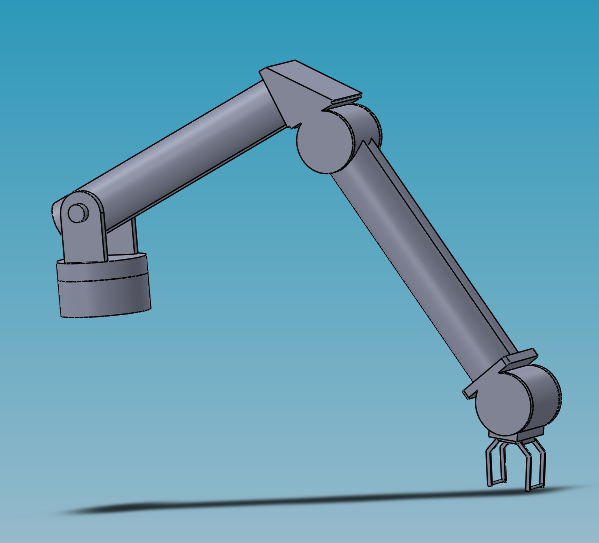
\includegraphics[scale=0.45]{sections/robot-design/images/arm_model.png}s
	\label{sample_return_rover:robot_design:arm_model}
	\caption{Arm Model in SolidWorks}
\end{figure}

\begin{figure}[H]
	\centering
	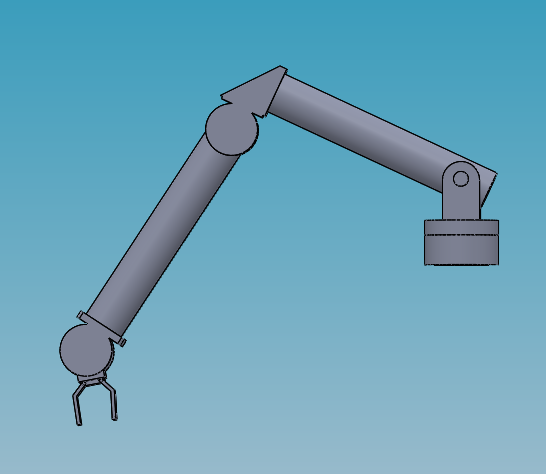
\includegraphics[scale=0.50]{sections/robot-design/images/arm_side.png}
	\label{sample_return_rover:robot_design:arm_side}
	\caption{Side View of Robot Arm}
\end{figure}
